\documentclass[a4paper,14pt]{extarticle}
\usepackage[top=1in,bottom=1in,left=1in,right=1in]{geometry}
\setlength{\emergencystretch}{2em}  % Allows some flexibility in line breaking
\usepackage{amsmath}
\usepackage{amssymb}
\usepackage{graphicx}
\usepackage{fontspec}
\usepackage{hyperref}
\usepackage{fontspec}

% Required packages
\usepackage{thmtools}
\usepackage{tikz}
\usepackage{xcolor}
\usepackage{mdframed}

% Define colors
\definecolor{contextcolor}{RGB}{240,248,255}  % Light blue
\definecolor{setupcolor}{RGB}{245,245,245}    % Light gray
\definecolor{thinkcolor}{RGB}{230,245,230}    % Light green

% Define counter for exercises
\newcounter{exercisecount}

% Define custom commands
\newcommand{\exercise}[1][]{%
    \stepcounter{exercisecount}%
    \phantomsection % Add anchor for hyperref
    \addcontentsline{toc}{section}{Exercise \theexercisecount: #1} % Add to table of contents
    \section*{\large\textbf{Exercise \theexercisecount:} #1}\par\medskip}

% Define custom commands
\newcounter{stepcount}[exercisecount]
\newcommand{\step}{\stepcounter{stepcount}\paragraph{Step \theexercisecount.\thestepcount}}
\newcommand{\think}[1]{
    \begin{mdframed}[backgroundcolor=thinkcolor,linewidth=0.5pt]
    \textit{Think:} #1
    \end{mdframed}}

% Document settings
\setlength{\parindent}{0pt}
\setlength{\parskip}{1em}

%\usetikzlibrary{decorations.pathmorphing}
\usetikzlibrary{calc,decorations,patterns,arrows,decorations.pathmorphing,positioning}
\definecolor{pltblue}{HTML}{1F77B4}
\tikzset{every picture/.style={/utils/exec={\fontspec{Pretty Neat}}}}
\setmainfont{Pretty Neat}

\usepackage{wasysym}  % Provides \Square symbol

\makeatletter
\pgfset{
  /pgf/decoration/randomness/.initial=2,
  /pgf/decoration/wavelength/.initial=100
}
\pgfdeclaredecoration{sketch}{init}{
  \state{init}[width=0pt,next state=draw,persistent precomputation={
    \pgfmathsetmacro\pgf@lib@dec@sketch@t0
  }]{}
  \state{draw}[width=\pgfdecorationsegmentlength,
  auto corner on length=\pgfdecorationsegmentlength,
  persistent precomputation={
    \pgfmathsetmacro\pgf@lib@dec@sketch@t{mod(\pgf@lib@dec@sketch@t+pow(\pgfkeysvalueof{/pgf/decoration/randomness},rand),\pgfkeysvalueof{/pgf/decoration/wavelength})}
  }]{
    \pgfmathparse{sin(2*\pgf@lib@dec@sketch@t*pi/\pgfkeysvalueof{/pgf/decoration/wavelength} r)}
    \pgfpathlineto{\pgfqpoint{\pgfdecorationsegmentlength}{\pgfmathresult\pgfdecorationsegmentamplitude}}
  }
  \state{final}{}
}
\tikzset{xkcd/.style={decorate,decoration={sketch,segment length=0.5pt,amplitude=0.5pt}}}
\makeatother

\usepackage{etoolbox}
\AtBeginEnvironment{tabular}{\fontspec{Pretty Neat}}

\setlength{\parindent}{0pt}
\setlength{\parskip}{0.5em}
\usepackage{fancyhdr}
\usepackage{geometry}
\usepackage{adjustbox}
\usepackage{titling}
\usepackage{multicol}
\usepackage{amsmath}
\usepackage{amssymb}
\usepackage{graphicx}
\usepackage{hyperref}
\usepackage{tikz}
\usepackage{fontspec}
\usetikzlibrary{calc,decorations,patterns,arrows,decorations.pathmorphing}
\definecolor{pltblue}{HTML}{1F77B4}

\usepackage{amsmath}
\usepackage{tikz}
\usepackage{enumitem}

\title{Random Walk Characteristics Worksheet}
\author{Network Science Course}
\date{}

\begin{document}


\exercise[Outer Product]

\step Calculate the outer product $\mathbf{a} \otimes \mathbf{b}$ for the vectors $\mathbf{a} = [1, 2, 3]$ and $\mathbf{b} = [1,3,1]$.
\think{How does each element in the first vector interact with each element in the second vector? Which elements of the resulting matrix become the largest?}

\vspace{3cm}

\step For each of the following vector pairs, visualize their outer product using shading patterns:
\begin{enumerate}
    \item $\mathbf{u} = [5,4,3,2,1]$ and $\mathbf{v} = [5,4,3,2,1]$
    \item $\mathbf{u} = [1,2,4,0,0]$ and $\mathbf{v} = [3, 1, 2, 0, 0]$
    \item $\mathbf{u} = [1,1,1,-1,-1]$ and $\mathbf{v} = [1,1,1,-1,-1]$
\end{enumerate}

\begin{center}
\begin{tabular}{ccc}
    (a) & (b) & (c) \\
    \begin{tabular}{|c|c|c|c|c|c|}
    \hline
    & 1 & 2 & 3 & 4 & 5 \\
    \hline
    1 & & & & & \\
    \hline
    2 & & & & & \\
    \hline
    3 & & & & & \\
    \hline
    4 & & & & & \\
    \hline
    5 & & & & & \\
    \hline
    \end{tabular}
    &
    \begin{tabular}{|c|c|c|c|c|c|}
    \hline
    & 1 & 2 & 3 & 4 & 5 \\
    \hline
    1 & & & & & \\
    \hline
    2 & & & & & \\
    \hline
    3 & & & & & \\
    \hline
    4 & & & & & \\
    \hline
    5 & & & & & \\
    \hline
    \end{tabular}
    &
    \begin{tabular}{|c|c|c|c|c|c|}
    \hline
    & 1 & 2 & 3 & 4 & 5 \\
    \hline
    1 & & & & & \\
    \hline
    2 & & & & & \\
    \hline
    3 & & & & & \\
    \hline
    4 & & & & & \\
    \hline
    5 & & & & & \\
    \hline
    \end{tabular}
\end{tabular}
\end{center}

\exercise[Matrix Decomposition]
\step Consider the following matrix representing a small network:
\[
\begin{bmatrix}
1 & 1 & 1 & 1 & 1 \\
1 & 1 & 1 & 1 & 1 \\
1 & 1 & 1 & 1 & 1 \\
1 & 1 & 1 & 1 & 1 \\
1 & 1 & 1 & 1 & 1
\end{bmatrix}
\]
Try to ``decompose'' this matrix into the outer product of two vectors with minimal error. Sketch the vectors and use shading to represent their values.
\vspace{3cm}

\step Now examine this more complex matrix:
\[
\begin{bmatrix}
8 & 4 & 2 & 1 & 0 \\
4 & 4 & 2 & 0 & 0 \\
2 & 2 & 2 & 1 & 0 \\
1 & 0 & 1 & 1 & 1 \\
0 & 0 & 0 & 1 & 1
\end{bmatrix}
\]
Can you decompose this into a sum of two outer products? Sketch the vectors for each outer product and use shading.
\vspace{3cm}

\step Building on your decomposition from Step 2:
If you had to keep only one of the two outer products, which would you choose and why? What information about the network would be preserved?
\vspace{3cm}

\exercise[Word Embeddings and Document Analysis]
\step Examine these short news headlines:
\begin{enumerate}
    \item ``Tech company launches new smartphone''
    \item ``Tech news update''
    \item ``Major tech company announces news update about smartphone technology advances''
    \item ``Smartphone sales rise in tech sector''
    \item ``New restaurant opens downtown''
    \item ``Local restaurant offers new menu''
\end{enumerate}

Count how many times each word appears in each headline and fill in the grid below:
\begin{center}
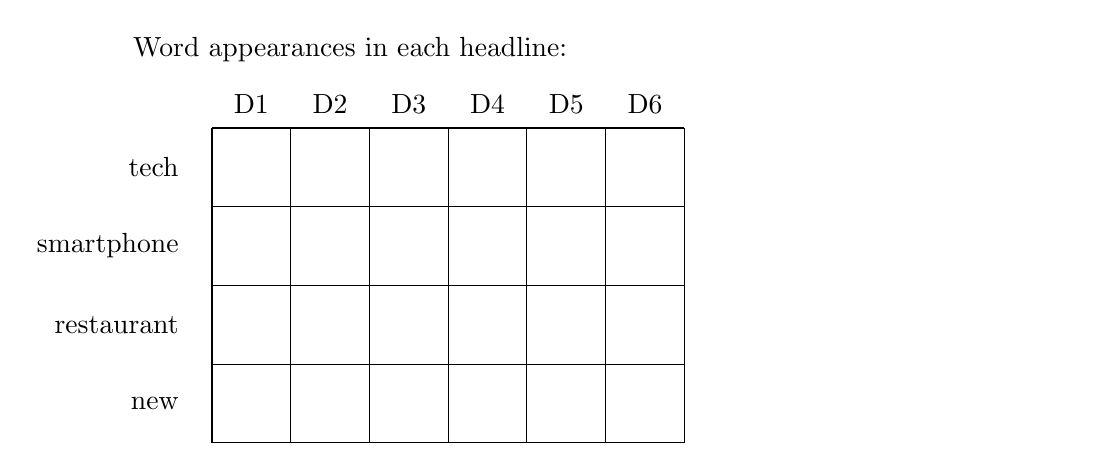
\begin{tikzpicture}
    % Create word-document matrix
    \node[text width=12cm] at (5,5) {Word appearances in each headline:};
    \begin{scope}[yshift=0cm]
        \draw (0,0) grid[step=1] (6,4);
        % Column headers (documents)
        \foreach \x/\t in {0.5/D1, 1.5/D2, 2.5/D3, 3.5/D4, 4.5/D5, 5.5/D6} {
            \node[rotate=0] at (\x,4.3) {\t};
        }
        % Row headers (words)
        \foreach \y/\t in {3.5/tech, 2.5/smartphone, 1.5/restaurant, 0.5/new} {
            \node[anchor=east] at (-0.3,\y) {\t};
        }
    \end{scope}
\end{tikzpicture}
\end{center}

\think{What patterns do you notice about how words are distributed across different types of headlines?}

\step Compare these two headlines:
\begin{enumerate}[label=\roman*.]
    \item Short headline: ``Tech news update''
    \item Longer headline: ``Major tech company announces news update about smartphone technology advances''
\end{enumerate}

\think{The word ``tech'' appears once in each headline. Why should these appearances be weighted differently? How does the length of each headline affect the significance of the word?}

\step Let's quantify word importance using term frequency (TF):
\[ \text{TF} = \frac{\text{number of times word appears in document}}{\text{total number of words in document}} \]

Calculate the TF for ``tech'' in both headlines:
\begin{center}
\begin{tabular}{|l|c|c|c|c|}
    \hline
    Headline & Word & Times & Total & Term \\
     & Count & Words & Frequency & (TF) \\
    \hline
    Short & & & & \\ \hline
    Long & & & & \\ \hline
\end{tabular}
\end{center}

\think{How does TF help capture the relative importance of words in documents of different lengths?}

\step Now let's consider how specific or general each word is across all documents using the inverse document frequency (IDF):
\[ \text{IDF} = \log\left(\frac{\text{total number of headlines}}{\text{number of headlines containing the word}}\right) \]

\begin{center}
\begin{tabular}{|l|c|c|}
    \hline
    Word & Appears in & IDF (Relative Specificity) \\
    & how many docs? & (darker = more specific) \\
    \hline
    tech & & \Square \\
    smartphone & & \Square \\
    restaurant & & \Square \\
    new & & \Square \\
    \hline
\end{tabular}
\end{center}

\think{What does IDF tell us about which words are topic-specific versus general-purpose?}

\step Combine TF and IDF to create word embeddings:
\[ \text{TF-IDF} = \text{TF} \times \text{IDF} \]

\begin{center}
    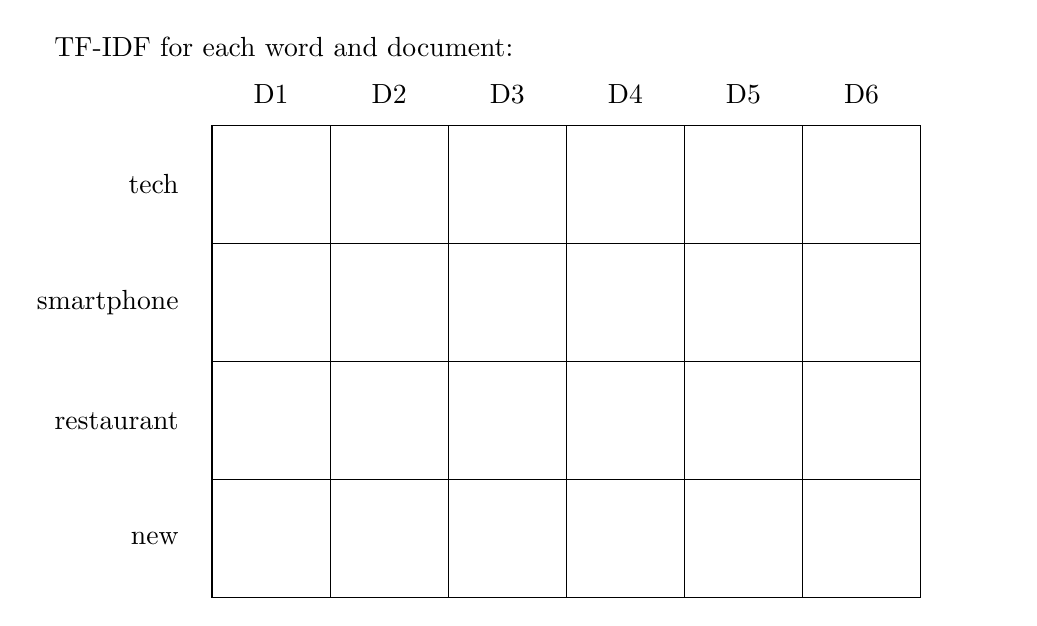
\begin{tikzpicture}
        % Create word-document matrix
        \node[text width=12cm] at (4,7) {TF-IDF for each word and document:};
        \begin{scope}[yshift=0cm]
            \draw (0,0) grid[step=1.5] (9,6);
            % Column headers (documents)
            \foreach \x/\t in {0.75/D1, 2.25/D2, 3.75/D3, 5.25/D4, 6.75/D5, 8.25/D6} {
                \node[rotate=0] at (\x,6.4) {\t};
            }
            % Row headers (words)
            \foreach \y/\t in {5.25/tech, 3.75/smartphone, 2.25/restaurant, 0.75/new} {
                \node[anchor=east] at (-0.3,\y) {\t};
            }
        \end{scope}
    \end{tikzpicture}
\end{center}

\think{How does TF-IDF combine the benefits of both TF and IDF to create more meaningful word representations?}

\step Decompose the TF-IDF matrix into meaningful components:
\begin{center}
    \begin{tikzpicture}
        % First matrix - original co-occurrence matrix
        \node at (2.5,5) {TF-IDF matrix};

        \draw (0,0) rectangle (5,4);
        \foreach \y in {1,2,3}
            \draw (0,\y) -- (5,\y);
        \foreach \x in {1,2,3,4}
            \draw (\x,0) -- (\x,4);

        % Multiplication symbol
        \node at (6,2) {$\simeq$};

        % Second matrix
        \node at (8,5) {Query matrix};
        \draw (7,0) rectangle (9,4);
        \draw (8,0) -- (8,4);
        \foreach \y in {1,2,3}
            \draw (7,\y) -- (9,\y);

        % Multiplication symbol
        \node at (10,2) {$\times$};

        % Third matrix
        \node at (13.5,5) {Key matrix};
        \draw (11,1) rectangle (17,3);
        \draw (11,2) -- (17,2);
        \foreach \x in {12,13,14,15,16}
            \draw (\x,1) -- (\x,3);
    \end{tikzpicture}
\end{center}

\think{What aspects of word/document meaning are captured by the query and key matrices?}

\step Visualize the word relationships in 2D space:
\vspace{-1cm}
\begin{center}
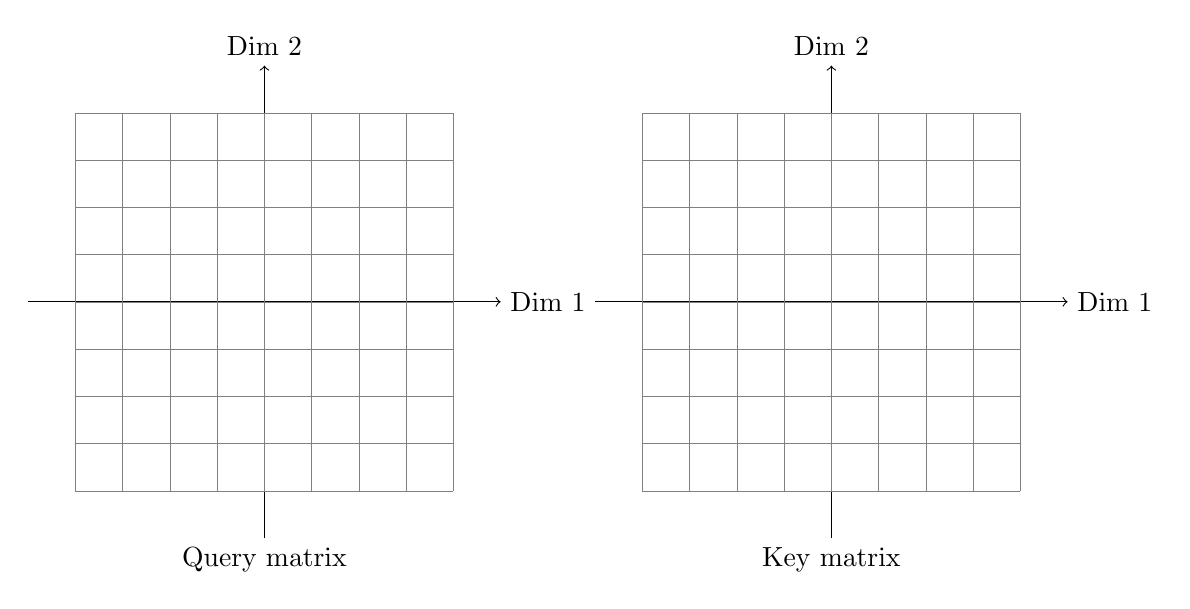
\begin{tikzpicture}[scale=0.6]
    % First grid
    \begin{scope}
        \draw[->] (-5,0) -- (5,0) node[right] {Dim 1};
        \draw[->] (0,-5) -- (0,5) node[above] {Dim 2};
        \draw[help lines] (-4,-4) grid (4,4);
        \node[below] at (0,-5) {Query matrix};
    \end{scope}

    % Second grid
    \begin{scope}[xshift=12cm]
        \draw[->] (-5,0) -- (5,0) node[right] {Dim 1};
        \draw[->] (0,-5) -- (0,5) node[above] {Dim 2};
        \draw[help lines] (-4,-4) grid (4,4);
        \node[below] at (0,-5) {Key matrix};
    \end{scope}
\end{tikzpicture}
\end{center}
\vspace{-1.5em}

Place "apple", "banana", and "curry" on the first matrix.
\think{What semantic relationships between words are revealed by their positions in the 2D space?}
\vspace{1.5cm}

\clearpage

\exercise[Pointwise Mutual Information]

\step Consider again our news headlines, but now let's look at which words appear together in the same headline. Create a word-word matrix:

\begin{center}
\begin{tikzpicture}
    \node[text width=12cm] at (5,7) {Word co-occurrences:};
    \begin{scope}[yshift=0cm]
        \draw (0,0) grid[step=1] (4,4);
        % Column and row headers (words)
        \foreach \x/\t in {0.5/tech, 1.5/smartphone, 2.5/restaurant, 3.5/new} {
            \node[rotate=90] at (\x,5.3) {\t};
            \node[anchor=east] at (-0.3,4-\x) {\t};
        }
    \end{scope}
\end{tikzpicture}
\end{center}

\think{What is the relationship between the word-document matrix and the word-word matrix?}

\step Consider the words "tech" and "smartphone". They appear together in 3 headlines (Probability of 3/6 = 0.5). If words appeared randomly, how many times would they appear together?
\vspace{3cm}

\step How about "tech" and "restaurant"? \vspace{3cm}

\step Calculate the expected co-occurrence and compare with observed:
\begin{center}
\begin{tabular}{|l|c|c|}
    \hline
    & tech-smartphone & tech-restaurant \\ \hline
    Observed co-occurrences &  &  \\ \hline
    Expected co-occurrences &  &  \\ \hline
    Ratio (Observed/Expected) &  &  \\ \hline
\end{tabular}
\end{center}

\think{What does it mean when the ratio is greater than 1? Less than 1?}

\step The Pointwise Mutual Information (PMI) is defined as:
\[ \text{PMI}(word1, word2) = \log\left(\frac{\text{P(word1, word2)}}{\text{P(word1) P(word2)}}\right) \]

where $P(word1, word2)$ is the probability of co-occurrence. It is the co-occurrence count divided by the sum of all co-occurrence counts. $P(word1)$ is the probability of word1 (e.g., 0.5 for "tech"), and $P(word2)$ is the probability of word2 (e.g., 0.5 for "smartphone"). Complete the PMI matrix for our words:
\begin{center}
\begin{tikzpicture}
    % Create PMI matrix with color scale
    \node[text width=12cm] at (4,7) {PMI values (darker = stronger positive association):};
    \begin{scope}[yshift=0cm]
        \draw (0,0) grid[step=1.5] (6,6);
        % Add labels and grid here
    \end{scope}
\end{tikzpicture}
\end{center}

\think{How does PMI capture different information than raw co-occurrence counts?}

\end{document}